\documentclass{article}

\title{Lab-exam}
\author{2347139}
\date{\today}


\usepackage{listings}
\usepackage{color}
\usepackage{graphicx}

\definecolor{dkgreen}{rgb}{0,0.6,0}
\definecolor{gray}{rgb}{0.5,0.5,0.5}
\definecolor{mauve}{rgb}{0.58,0,0.82}

\lstset{frame=tb,
  language=Java,
  aboveskip=3mm,
  belowskip=3mm,
  showstringspaces=false,
  columns=flexible,
  basicstyle={\small\ttfamily},
  numbers=left,
  numberstyle=\tiny\color{gray},
  keywordstyle=\color{blue},
  commentstyle=\color{dkgreen},
  stringstyle=\color{mauve},
  breaklines=true,
  breakatwhitespace=true,
  tabsize=3
}
\begin{document}
\maketitle
\begin{lstlisting}
  
interface studeInter {
    public void firstClass();

    public void checkAttendence();

}

abstract class Person {
    String name;
    int age;
    int height;

    public void get(String name, int age, int height) {
        this.name = name;
        this.age = age;
        this.height = height;
    }

    public void show() {
        System.out.println("Name of the Person is " + name);
        System.out.println("Age of the Person" + name + "is" + age);
        System.out.println("height of the Person" + name + "is" + height);
    }

    abstract void formatDOB(int d, int m, int y);
}

class Student extends Person {
    static int studId;
    String institutionName;
    double phoneNumber;

    public void get(String institutionName, double phoneNumber) {
        this.institutionName = institutionName;
        this.phoneNumber = phoneNumber;
    }

    public void show() {
        System.out.println("Student id is " + studId);

        System.out.println("institution Name of the student " + studId + "is" + age);
        System.out.println("Phone number of the student ID " + studId + " is " + phoneNumber);
    }

    void formatDOB(int d, int m, int y) {
        int today = 2023;
        int age = today - y;
        System.out.println("Calculated age of the student from DOB is" + age);
    }
}

class GraduateStudent extends Student implements studeInter {

    GraduateStudent() {
        super.show();
    }

    final String programName = "MCA";
    int noOfSubjects;
    String classTeacherName;
    int marks;
    int attendance;

    public void get(int noOfSubjects, String classTeacherName, int marks, int attendance) {
        // this.programName = programName;
        this.noOfSubjects = noOfSubjects;
        this.classTeacherName = classTeacherName;
        this.marks = marks;
        this.attendance = attendance;

    }

    public void show() {
        System.out.println("The program name is " + programName);
        System.out.println("Number of subjects in the program " + noOfSubjects);
        System.out.println("Class teacher name " + classTeacherName);
        System.out.println("Marks " + marks);
        System.out.println("Have enough attendence" + attendance);

    }

    public void firstClass() {
        if (marks >= 60) {
            show();
        }
    }

    public void checkAttendence() {
        if (marks >= 75) {
            show();
        }
    }

}

class Main {
    public static void main(String[] args) {
        Student[] stud;
        stud = new Student[5];

        stud[0] = new Student();
        Student.studId = 01;
        stud[0].get("christ university", 988658954);
        stud[0].show();

        stud[1] = new Student();
        Student.studId = 02;
        stud[1].get("SJC", 988658954);
        stud[1].show();

        stud[2] = new Student();
        Student.studId = 02;
        stud[2].get("PES university", 989989876);
        stud[2].show();

        stud[3] = new Student();
        Student.studId = 03;
        stud[3].get("Bishop cottons", 988658954);
        stud[3].show();

        stud[4] = new Student();
        Student.studId = 04;
        stud[4].get("Kristu jayanthi", 988658954);
        stud[4].show();

        // graduate Student
        GraduateStudent[] gStud;
        gStud = new GraduateStudent[4];

        gStud[0] = new GraduateStudent();
        gStud[0].get(7, "abc", 65, 75);
        // gStud[0].show();
        gStud[0].firstClass();
        gStud[0].checkAttendence();

    }
}
\end{lstlisting}

\section*{Output}
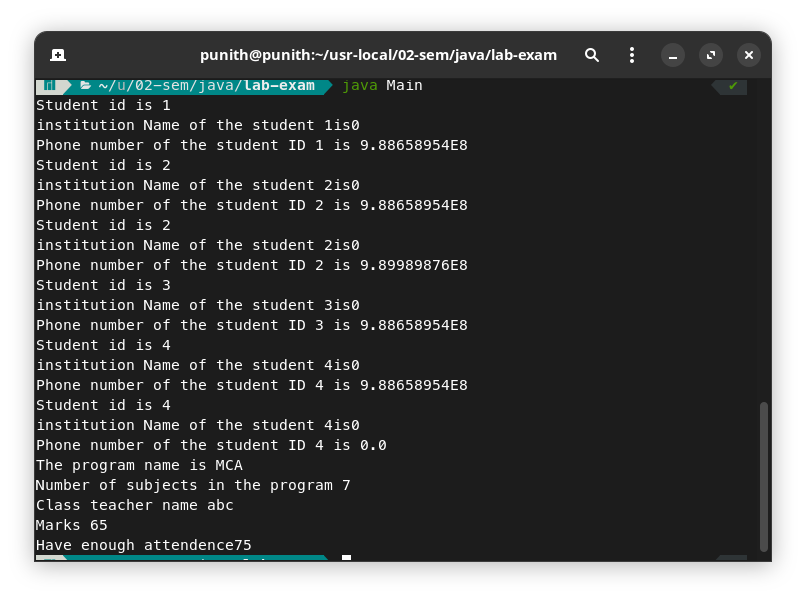
\includegraphics[width=11cm, height=9cm]{./images/01.png}

\end{document}
